\section{Trzecia metoda (Metoda19)}
\subsection{Pomysł na metodę}
Metoda19 jest efektem rozwoju pomysłów z Metoda5 i Metoda9, które opierały się na
algorytmach drzewiastych i metodach integracji wyników. W Metoda5
zastosowano Random Forest i XGBoost jako modele bazowe, które następnie
były integrowane za pomocą regresji logistycznej. W Metoda9 kluczową rolę
odgrywał Random Forest jako jeden z głównych komponentów
VotingClassifier, co podkreśliło jego efektywność w różnorodnych
konfiguracjach.

W Metoda19 połączono Random Forest i Extra Trees, dwa modele bazowe
opierające się na konstrukcji drzew decyzyjnych. Extra Trees, w
przeciwieństwie do Random Forest, wprowadza dodatkowy element losowości
w wyborze punktów podziału, co zwiększa różnorodność wyników. Inspiracja
pochodząca z Metoda5 była widoczna w zastosowaniu regresji logistycznej
jako meta-modelu, który skutecznie integruje predykcje obu modeli. Metoda19
dodatkowo rozwija te pomysły, kładąc nacisk na stabilność wyników dzięki
różnorodności predykcji generowanych przez Random Forest i Extra Trees.

\subsection{Wejściowe dane}
Metoda train\_run19 przyjmuje następujące parametry wejściowe:

\begin{enumerate}
\def\labelenumi{\arabic{enumi}.}
\item
  \textbf{X\_train}: Macierz danych treningowych, gdzie każdy wiersz to
  jedna próbka, a kolumny to cechy. Rozmiar: \textbf{n × m}, gdzie
  \textbf{n} to liczba próbek, a \textbf{m} to liczba cech.
\item
  \textbf{y\_train}: Wektor etykiet dla danych treningowych. Rozmiar:
  \textbf{n,} gdzie \textbf{n} to liczba próbek w danych treningowych.
\item
  \textbf{X\_test}: Macierz danych testowych, analogiczna do
  \textbf{X\_train}, używana do oceny modelu.
\item
  \textbf{y\_test}: Wektor etykiet testowych, odpowiadający danym
  testowym.
\end{enumerate}

\subsection{Wyjściowe dane}
Metoda zwraca następujące elementy:

\begin{enumerate}
\def\labelenumi{\arabic{enumi}.}
\item
  \textbf{meta\_model}: Meta-model wytrenowany na danych pochodzących z
  predykcji modeli \textbf{Random Forest} i \textbf{Extra Trees.}
\item
  \textbf{meta\_features\_test}: Macierz meta-cech, zbudowana na
  podstawie predykcji modeli bazowych dla danych testowych.
\item
  \textbf{y\_test}: Wektor etykiet testowych, identyczny z wejściowym
  \textbf{y\_test}.
\end{enumerate}

\subsection{Algorytm}
\begin{enumerate}
\def\labelenumi{\arabic{enumi}.}
\item
  Trenowanie modeli bazowych:

  \begin{itemize}
  \item
    \textbf{Random Forest}:

    \begin{itemize}
    \item
      Model \textbf{RandomForestClassifier} jest inicjalizowany z
      \textbf{100 estymatorami} i \textbf{stanem losowości
      (random\_state) 42}.
    \item
      Model jest trenowany na danych treningowych \textbf{X\_train} i
      \textbf{y\_train}.
    \end{itemize}
  \item
    \textbf{Extra Trees}:

    \begin{itemize}
    \item
      Model \textbf{ExtraTreesClassifier} jest inicjalizowany z
      \textbf{100 estymatorami} i \textbf{stanem losowości
      (random\_state) 4}2.
    \item
      Model jest trenowany na tych samych danych treningowych.
    \end{itemize}
  \end{itemize}
\item
  Generowanie predykcji dla danych treningowych:

  \begin{itemize}
  \item
    Obliczane są prawdopodobieństwa klasy pozytywnej \textbf{\( P(y=1 \mid x) \)} dla obu modeli bazowych:

    \begin{itemize}
    \item
      \textbf{rf\_preds\_train}: \textbf{Predykcje Random Forest}.
    \item
      \textbf{et\_preds\_train}: \textbf{Predykcje Extra Trees}.
    \end{itemize}
  \item
    Predykcje są używane do stworzenia macierzy meta-cech, gdzie kolumny
    to \textbf{rf\_\allowbreak preds} i \textbf{et\_\allowbreak preds}.
  \end{itemize}
\item
  Trenowanie meta-modelu:

  \begin{itemize}
  \item
    Wytrenowany na \textbf{danych} \textbf{meta-cech,
    meta\_features\_train}, oraz rzeczywistych etykietach
    \textbf{y\_train}.
  \item
    Meta-modelem jest \textbf{regresja logistyczna, LogisticRegression},
    która łączy predykcje obu modeli bazowych.
  \end{itemize}
\item
  Generowanie predykcji dla danych testowych:

  \begin{itemize}
  \item
    Obliczane są prawdopodobieństwa klasy pozytywnej dla \textbf{Random
    Forest} i \textbf{Extra Trees}:

    \begin{itemize}
    \item
      \textbf{rf\_preds\_test}: \textbf{Predykcje Random Forest}.
    \item
      \textbf{et\_preds\_test}: \textbf{Predykcje Extra Trees}.
    \end{itemize}
  \item
    Tworzona jest \textbf{macierz meta-cech} dla danych testowych,
    analogiczna struktura jak dla danych treningowych.
  \end{itemize}
\item
  Zwracanie wyników: meta-model, macierz meta-cech dla testu oraz
  etykiety testowe są zwracane.
\end{enumerate}

\subsection{Kod}
\begin{lstlisting}[caption={Kod do 19 metody}, label={19Metoda}]
rf_clf = RandomForestClassifier(
    n_estimators=100, 
    random_state=42
)  # Random Forest
et_clf = ExtraTreesClassifier(
    n_estimators=100, 
    random_state=42
)  # Extra Trees
rf_clf.fit(X_train, y_train)
et_clf.fit(X_train, y_train)
rf_preds_train = rf_clf.predict_proba(X_train)[:, 1] 
et_preds_train = et_clf.predict_proba(X_train)[:, 1] 
meta_features_train = pd.DataFrame({ 
    'rf_preds': rf_preds_train,
    'et_preds': et_preds_train
})
meta_model = LogisticRegression() 
meta_model.fit(meta_features_train, y_train)
rf_preds_test = rf_clf.predict_proba(X_test)[:, 1]
et_preds_test = et_clf.predict_proba(X_test)[:, 1] 
meta_features_test = pd.DataFrame({ 
    'rf_preds': rf_preds_test,
    'et_preds': et_preds_test
})
return meta_model, meta_features_test, y_test
\end{lstlisting}

\subsection{Schemat blokowy}
\begin{figure}[H]
	\centering
	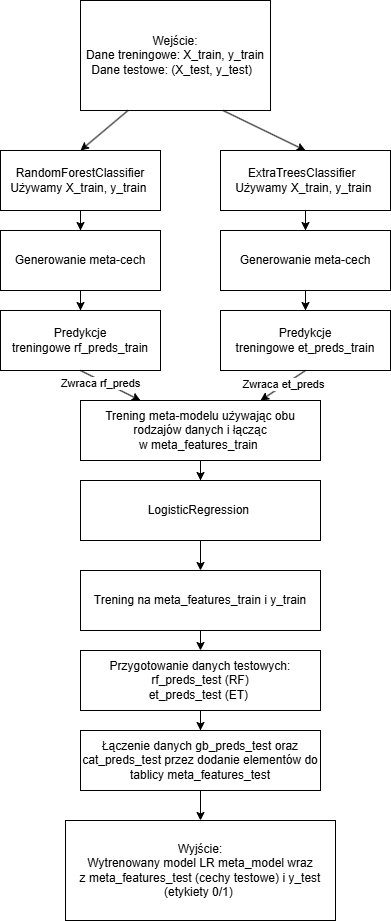
\includegraphics[width=0.5\textwidth]{img/diagrams/metoda19.drawio.png}
	\caption{Schemat metody 19.}
	\label{fig:diagram_metoda19}
\end{figure}

\subsection{Właściwości analityczne}
\begin{enumerate}
\def\labelenumi{\arabic{enumi}.}
\item
  \textbf{Efektywność}:

  \begin{itemize}
  \item
    \textbf{Random Forest} i \textbf{Extra Trees} bazują na zbiorach
    drzew decyzyjnych, które są w stanie uchwycić zarówno zależności
    liniowe, jak i nieliniowe.
  \item
    Meta-model, w podanej implementacji \textbf{regresja logistyczna},
    umożliwia dodatkową poprawę wyników dzięki łączeniu predykcji z
    modeli bazowych.
  \end{itemize}
\item
  \textbf{Elastyczność}: metoda może być łatwo dostosowana do różnych
  problemów klasyfikacyjnych i różnorodnych zbiorów danych.
\item
  \textbf{Stabilność}:

  \begin{itemize}
  \item
    Modele bazowe, takie jak \textbf{Random Forest} i \textbf{Extra
    Trees}, są naturalnie stabilne dzięki losowemu wybieraniu próbek i
    cech podczas tworzenia drzew.
  \item
    Meta-model dodatkowo redukuje wariancję wyników, zwiększając
    spójność predykcji.
  \end{itemize}
\item
  \textbf{Złożoność obliczeniowa}:

  \begin{itemize}
  \item
    Zarówno \textbf{Random Forest}, jak i \textbf{Extra Trees} mają
    złożoność liniową względem liczby próbek i liczby estymatorów, co
    pozwala na efektywne przetwarzanie dużych zbiorów danych.
  \item
    Regresja logistyczna jako meta-model jest szybka i wydajna, dzięki
    czemu metoda jest odpowiednia nawet dla dużych zbiorów danych.
  \end{itemize}
\item
  \textbf{Wydajność}: \textbf{Random Forest} i \textbf{Extra Trees} są
  zoptymalizowane do przetwarzania dużych zbiorów danych i cech o różnym
  typie. Ich kombinacja pozwala na uzyskanie bardziej dokładnych
  wyników.
\end{enumerate}